Chương này trình bày quá trình hiện thực hoá và đánh giá hệ thống GraphRAG đã được thiết kế ở Chương 3. Nội dung được tổ chức thành ba phần: cài đặt hệ thống, thực nghiệm định lượng và triển khai kèm kiểm nghiệm với người dùng.

\section{Cài đặt và phát triển hệ thống}
\label{sec:system_setup}

Hệ thống được phát triển trên máy cá nhân chạy Windows và đóng gói để triển khai trên Google Cloud Run phục vụ giai đoạn kiểm nghiệm với người dùng (Mục~\ref{sec:user_deployment}). Knowledge Graph Chèo được dựng trên Neo4j theo quy trình đã trình bày ở Mục~3.2, gồm bảy vở chèo cổ, 38 nhân vật, 41 diễn viên, 15 trích đoạn và 27 phiên bản biểu diễn; pipeline GraphRAG với cả ba chiến lược tạo sinh Pre/Mid/Post-Generation (Mục~3.3.2) được hiện thực hoá đầy đủ và có thể chuyển đổi qua cấu hình. Mô hình ngôn ngữ lớn được sử dụng qua API để đảm bảo tính \textit{LLM-agnostic} (Mục~3.1.1); một mô hình duy nhất được chọn làm mô hình chính cho toàn bộ thực nghiệm với tham số sinh cố định (temperature bằng 0, top-p bằng 1) để đảm bảo khả năng tái lập.

Ngoài GraphRAG, hai hệ thống tham chiếu được triển khai làm đối chứng cho các thí nghiệm so sánh ở Mục~\ref{sec:experiments}. Hệ thống thứ nhất là \textbf{RAG truyền thống}: tài liệu mô tả nghệ thuật Chèo được chia thành các đoạn văn bản có độ dài cố định, nhúng véc-tơ bằng một mô hình embedding và lưu trong vector store; khi nhận câu hỏi, hệ thống tính độ tương đồng cosine giữa véc-tơ câu hỏi và toàn bộ véc-tơ đoạn văn, lấy một số đoạn gần nhất làm ngữ cảnh trước khi gửi tới mô hình ngôn ngữ. Hệ thống thứ hai là \textbf{LLM-only}: câu hỏi được gửi trực tiếp tới mô hình ngôn ngữ kèm một prompt hệ thống ngắn xác định miền nghệ thuật Chèo, không có cơ chế truy xuất; baseline này tách biệt đóng góp của cơ chế truy xuất so với tri thức nội tại của mô hình.

Cả ba hệ thống chia sẻ cùng mô hình ngôn ngữ và cùng tham số sinh để chênh lệch kết quả chỉ phản ánh khác biệt về nguồn tri thức và cơ chế truy xuất. Prompt của RAG truyền thống và LLM-only được thiết kế đơn giản, chỉ yêu cầu trả lời bằng tiếng Việt dựa trên ngữ cảnh được cung cấp nếu có, không áp dụng các ràng buộc cấu trúc như trong ba chiến lược tạo sinh của GraphRAG. Cách thiết kế này giữ cho các baseline phản ánh đúng đặc trưng gốc, tránh việc kết quả được cải thiện một cách nhân tạo bởi các kỹ thuật prompting nâng cao.

\section{Thực nghiệm}
\label{sec:experiments}

\subsection{Mục tiêu và câu hỏi nghiên cứu}

Thực nghiệm nhằm đánh giá một cách định lượng hiệu quả của kiến trúc GraphRAG đề xuất đối với việc khai thác tri thức có cấu trúc trong miền nghệ thuật Chèo, đồng thời phân tích lợi ích của việc tích hợp Knowledge Graph so với hệ thống Retrieval-Augmented Generation truyền thống dựa trên truy xuất văn bản. Trên cơ sở đó, ba câu hỏi nghiên cứu được xác lập:

\begin{itemize}
  \item \textbf{RQ1.} Kiến trúc GraphRAG có cải thiện chất lượng truy xuất và chất lượng tạo sinh so với hệ thống RAG truyền thống trong miền nghệ thuật Chèo hay không, và ở mức độ nào?
  \item \textbf{RQ2.} Lợi ích của GraphRAG thay đổi thế nào theo độ phức tạp của truy vấn, từ truy vấn cục bộ (Local) tới truy vấn yêu cầu tổng hợp toàn cục (Global)?
  \item \textbf{RQ3.} Từng mức độ truy xuất trong Knowledge Graph (node, triplet, path, tiểu đồ thị) đóng góp ra sao vào hiệu năng tổng thể, và việc kết hợp đa mức độ có tạo ra lợi ích vượt trên từng mức độ riêng lẻ hay không?
\end{itemize}

\subsection{Kiểm chứng tính hợp lệ của CheoBench v2}
\label{sec:benchmark_validity}

Tính hợp lệ của bộ dữ liệu được đánh giá trên bốn chiều theo khung Messick~\cite{messick1995validity}: bao phủ nội dung, cấu trúc độ khó, khả năng phân biệt hệ thống và nhất quán của hệ độ đo. Số liệu được tính từ bộ câu hỏi và từ kết quả 100 câu ở Mục~\ref{sec:experiments}.

Về bao phủ nội dung, 100 câu hỏi liệt kê 225 thực thể trong trường \texttt{related\_entities}; đối chiếu với Knowledge Graph, bộ câu hỏi phủ 7/7 vở chèo, 24/38 nhân vật, 23/41 diễn viên và 9/15 trích đoạn (Bảng~\ref{tab:coverage_entity}). Toàn bộ 225 thực thể đều khớp với định danh trong KG, không câu nào yêu cầu tri thức ngoài phạm vi hệ thống. Coverage ở lớp vở đạt 100\%; các lớp con dao động từ 56\% đến 63\%, tập trung vào các thực thể trung tâm theo thực hành của BEIR~\cite{thakur2021beir}. 100 câu hỏi được phân vào 10 subcategory khác nhau, trải trên nhiều dạng truy vấn.

\begin{table}[h]
\centering
\caption{Mức độ bao phủ của CheoBench v2 trên Knowledge Graph Chèo.}
\label{tab:coverage_entity}
\begin{tabular}{lrrr}
\hline
\textbf{Loại thực thể} & \textbf{Đã phủ} & \textbf{Tổng} & \textbf{Tỷ lệ} \\
\hline
Vở chèo       &  7 &  7 & 100.0\% \\
Nhân vật      & 24 & 38 &  63.2\% \\
Diễn viên     & 23 & 41 &  56.1\% \\
Trích đoạn    &  9 & 15 &  60.0\% \\
\hline
\end{tabular}
\end{table}

Về cấu trúc độ khó, Edge et al.~\cite{edge2024graphrag} dự đoán khoảng cách GraphRAG--RAG giảm dần từ truy vấn Local (ánh xạ tên riêng) đến truy vấn Global (tổng hợp toàn cục). Bảng~\ref{tab:construct_validity} xác nhận xu hướng này trên 100 câu hỏi: khoảng cách giảm đơn điệu từ +0,309 (Local) qua +0,245 (Community) xuống +0,163 (Global). Số thực thể liên quan trung bình cũng phân tách ba nhóm ở mức 1,94 (Local), 2,50 (Community) và 2,33 (Global).

\begin{table}[h]
\centering
\caption{Khoảng cách hiệu năng GraphRAG--RAG theo nhóm truy vấn.}
\label{tab:construct_validity}
\begin{tabular}{lcccc}
\hline
\textbf{Nhóm} & \textbf{\#Ents TB} & \textbf{GraphRAG} & \textbf{RAG} & \textbf{Khoảng cách} \\
\hline
Local      & 1.94 & 0.862 & 0.553 & +0.309 \\
Community  & 2.50 & 0.861 & 0.616 & +0.245 \\
Global     & 2.33 & 0.782 & 0.619 & +0.163 \\
\hline
\end{tabular}
\end{table}

Về khả năng phân biệt hệ thống, trên 100 cặp (GraphRAG, RAG) không có cặp hoà điểm, 94 cặp GraphRAG đạt điểm cao hơn, $\Delta = S_{\text{GraphRAG}} - S_{\text{RAG}}$ có trung bình +0,240 và độ lệch chuẩn 0,193. Phân phối trải rộng với 72\% cặp có $|\Delta| \geq 0{,}10$ và 33\% cặp có $|\Delta| \geq 0{,}30$ (Bảng~\ref{tab:discrimination}), cho phép phân biệt hai hệ thống ở nhiều cấp độ thay vì ở hai cực.

\begin{table}[h]
\centering
\caption{Phân phối khoảng cách điểm tổng hợp $\Delta = S_{\text{GraphRAG}} - S_{\text{RAG}}$ trên 100 câu hỏi.}
\label{tab:discrimination}
\begin{tabular}{lrr}
\hline
\textbf{Chỉ số} & \textbf{Giá trị} & \textbf{Tỷ lệ} \\
\hline
Câu có GraphRAG $\geq$ RAG & 94/100 & 94.0\% \\
Câu hoà điểm ($|\Delta| < 10^{-6}$) &  0/100 &  0.0\% \\
Câu có $|\Delta| \geq 0.05$ & 84/100 & 84.0\% \\
Câu có $|\Delta| \geq 0.10$ & 72/100 & 72.0\% \\
Câu có $|\Delta| \geq 0.20$ & 50/100 & 50.0\% \\
Câu có $|\Delta| \geq 0.30$ & 33/100 & 33.0\% \\
\hline
Trung bình $\Delta$ & +0.240 & --- \\
Độ lệch chuẩn của $\Delta$ &  0.193 & --- \\
\hline
\end{tabular}
\end{table}

Về nhất quán của hệ độ đo, Cronbach's $\alpha$~\cite{cronbach1951alpha} tính trên điểm per-case của GraphRAG cho khối IR năm độ đo (MAP, NDCG@10, Precision, Recall, ContextEntitiesRecall) đạt 0,790, vượt ngưỡng 0,70~\cite{nunnally1978psychometric}; $\alpha$ toàn cục chín độ đo là 0,699 (Bảng~\ref{tab:consistency}). Hai khối Context và Generation có $\alpha$ gần 0, cho thấy các cặp độ đo trong mỗi khối đo các khía cạnh khác nhau (độ liên quan so với độ bao phủ; độ trung thực so với độ phù hợp). Tương quan Pearson bổ sung: $r(\text{MAP}, \text{NDCG@10}) = 0{,}98$, Faithfulness trực giao với các độ đo khác ($|r| \leq 0{,}06$), ContextEntitiesRecall tương quan yếu với mọi độ đo ($|r| \leq 0{,}14$). Bộ chín độ đo do đó vừa có khối nhất quán nội tại, vừa có các chiều bổ sung trực giao.

\begin{table}[h]
\centering
\caption{Cronbach's $\alpha$ của các khối độ đo trên 100 câu hỏi (hệ thống GraphRAG).}
\label{tab:consistency}
\begin{tabular}{lcc}
\hline
\textbf{Khối độ đo} & \textbf{Số độ đo} & \textbf{Cronbach's $\alpha$} \\
\hline
Toàn bộ                   & 9 & 0.699 \\
Khối IR xác định          & 5 & \textbf{0.790} \\
Khối Context (RAGAs)      & 2 & $-0.048$ \\
Khối Generation (RAGAs)   & 2 & $-0.063$ \\
\hline
\end{tabular}
\end{table}

\subsection{Thiết kế thực nghiệm}

Thiết kế dựa trên ba nguyên tắc: \textit{kiểm soát biến} --- mọi cấu hình không liên quan đến đối tượng so sánh đều được giữ cố định; \textit{đánh giá đa chiều} --- đồng thời đo chất lượng truy xuất và chất lượng tạo sinh; \textit{phân tích phân nhóm} --- kết quả được tách riêng theo ba nhóm truy vấn để làm rõ vị thế của GraphRAG trên các mức độ phức tạp khác nhau.

Thực nghiệm sử dụng toàn bộ 100 câu hỏi của CheoBench v2, phân thành ba nhóm Local (35 câu), Community (32 câu) và Global (33 câu) (Mục 3.4). Hai hệ thống tham gia so sánh gồm GraphRAG với pipeline truy xuất đa mức độ trên Knowledge Graph và RAG truyền thống sử dụng vector search trên văn bản. Cả hai chia sẻ cùng một mô hình ngôn ngữ và cùng bộ tham số sinh (Mục~\ref{sec:system_setup}); khác biệt duy nhất nằm ở nguồn tri thức và cơ chế truy xuất, nhờ vậy mọi chênh lệch quan sát được đều phản ánh đúng ảnh hưởng của hai thành phần này.

Đối với câu hỏi về mức độ truy xuất (RQ3), thực nghiệm ablation được thiết kế riêng: GraphRAG được cấu hình lần lượt sử dụng đúng một mức truy xuất (node, triplet, path hoặc tiểu đồ thị), rồi so sánh với cấu hình kết hợp đa mức độ. Tất cả năm cấu hình chia sẻ cùng định dạng ngữ cảnh và chiến lược tạo sinh mặc định; chênh lệch duy nhất nằm ở cơ chế truy xuất. Để kiểm soát chi phí gọi mô hình ngôn ngữ khi phải chạy năm cấu hình, ablation sử dụng tập con 20 câu phân tầng theo ba nhóm truy vấn (bảy câu Local, bảy câu Community, sáu câu Global), với cùng tập câu được dùng cho cả năm cấu hình nhằm đảm bảo so sánh công bằng.

\subsection{Độ đo đánh giá}
\label{sec:metrics}

\subsubsection{Chất lượng truy xuất}

Chất lượng truy xuất được đánh giá bởi bảy độ đo chia thành hai nhóm theo cách tính. Nhóm thứ nhất là các độ đo \textbf{xác định}, tính trực tiếp từ so sánh giữa kết quả truy xuất và ground truth, có thể tái lập chính xác giữa các lần chạy. Nhóm thứ hai là các độ đo \textbf{do mô hình ngôn ngữ chấm điểm} (LLM-as-judge), phản ánh các khía cạnh ngữ nghĩa mà công thức đối sánh chuỗi không biểu diễn được, với biến động nhỏ giữa các lần chạy được kiểm soát bằng cách cố định \texttt{temperature} ở 0.

Năm độ đo xác định được triển khai như sau:

\begin{itemize}
  \item \textbf{MAP}~\cite{manning2008ir} --- trung bình độ chính xác (average precision) trên toàn bộ truy vấn; trong bài toán này, MAP thưởng các cấu hình đưa nhiều thực thể đúng lên vị trí đầu của danh sách truy xuất, phản ánh chất lượng xếp hạng tổng thể.

  \item \textbf{NDCG@10}~\cite{jarvelin2002ndcg} --- đánh giá chất lượng xếp hạng ở mười vị trí đầu với phạt logarit theo vị trí; mức cắt $K = 10$ được chọn để phù hợp với kích thước ngữ cảnh điển hình mà pipeline đưa vào mô hình ngôn ngữ.

  \item \textbf{Precision} và \textbf{Recall} --- tỷ lệ chính xác và độ bao phủ của kết quả truy xuất so với tập thực thể liên quan $R$ theo ground truth, tính trên toàn bộ danh sách truy xuất $L$ sau khi loại trùng lặp:
    \begin{equation}
      \text{Precision} = \frac{|L \cap R|}{|L|}, \qquad \text{Recall} = \frac{|L \cap R|}{|R|}.
    \end{equation}

  \item \textbf{Context Entities Recall} --- tỷ lệ các thực thể bắt buộc theo ground truth xuất hiện trong ngữ cảnh đã được truy xuất. Gọi $E$ là tập thực thể bắt buộc (lấy trực tiếp từ trường \texttt{related\_entities} của CheoBench v2):
    \begin{equation}
      \text{Context Entities Recall} = \frac{|E \cap \text{context}|}{|E|}.
    \end{equation}
\end{itemize}

Hai độ đo do mô hình ngôn ngữ chấm điểm thuộc họ RAGAs~\cite{es2023ragas}, đều nằm trong thang $[0, 1]$ và được ước lượng trực tiếp qua lời gọi mô hình:

\begin{itemize}
  \item \textbf{Context Precision} --- mô hình được đưa cặp (câu hỏi, ngữ cảnh) và ước lượng tỷ lệ thông tin trong ngữ cảnh thực sự liên quan đến câu hỏi.

  \item \textbf{Context Recall} --- mô hình được đưa cặp (ground truth, ngữ cảnh) và ước lượng mức độ thông tin trong ground truth được ngữ cảnh bao phủ.
\end{itemize}

Điểm truy xuất tổng hợp được tính theo công thức:

\begin{equation}
\begin{aligned}
S_{\text{retrieval}} =\;& 0.20 \cdot \text{MAP}
  + 0.15 \cdot \text{NDCG@10} \\
& + 0.10 \cdot \text{Precision}
  + 0.10 \cdot \text{Recall} \\
& + 0.20 \cdot \text{Context Precision}
  + 0.15 \cdot \text{Context Recall} \\
& + 0.10 \cdot \text{Context Entities Recall}.
\end{aligned}
\end{equation}

Việc phân bổ trọng số tuân theo ba nguyên tắc. Trước hết, khối IR xác định nhận tổng 0,55 cao hơn khối RAGAs (0,45), do các độ đo IR có thể tính toán trực tiếp và tái lập chính xác, trong khi RAGAs phụ thuộc vào phán đoán của mô hình ngôn ngữ và chịu biến động nhỏ giữa các lần chạy. Tiếp theo, trong khối IR, MAP giữ trọng số cao nhất (0,20) do bao quát toàn bộ chất lượng xếp hạng trên mọi vị trí, NDCG@10 đứng thứ hai (0,15) do chỉ nhạy với mười vị trí đầu, còn Precision và Recall mỗi độ đo chỉ phản ánh một khía cạnh riêng --- chính xác hoặc bao phủ --- nên được cân bằng ở 0,10. Cuối cùng, trong khối RAGAs, Context Precision được ưu tiên cao nhất (0,20) vì ngữ cảnh chứa thông tin không liên quan dễ dẫn mô hình ngôn ngữ đi lệch hướng và ảnh hưởng trực tiếp đến chất lượng câu trả lời, trong khi Context Recall (0,15) và Context Entities Recall (0,10) cùng đo độ bao phủ nhưng ở các phạm vi khác nhau, với Entities Recall hẹp hơn nên nhận trọng số thấp hơn.

Cơ chế tổng hợp xử lý trường hợp độ đo không khả dụng bằng tái chuẩn hoá. Khi một độ đo RAGAs trả về giá trị vô hiệu do lỗi tạm thời của mô hình, độ đo đó được loại khỏi công thức và các trọng số còn lại được chuẩn hoá lại về tổng 1. Điểm truy xuất do đó luôn được tính trên tập độ đo khả dụng cho từng câu hỏi, tránh việc lỗi kỹ thuật đơn lẻ làm giảm kết quả đánh giá.

\subsubsection{Chất lượng tạo sinh}

Chất lượng tạo sinh được đánh giá qua hai độ đo RAGAs~\cite{es2023ragas}, \textbf{cả hai đều thuộc loại LLM-as-judge} --- mô hình ngôn ngữ đóng vai trò bên chấm điểm và trả về giá trị trong thang $[0, 1]$. \textbf{Faithfulness} đo tỷ lệ nội dung câu trả lời thực sự được ngữ cảnh truy xuất hỗ trợ, được thiết kế để phát hiện hallucination --- hiện tượng mô hình ngôn ngữ đưa ra thông tin không có trong ngữ cảnh. Giá trị của độ đo được tính qua hai bước, mỗi bước là một lời gọi mô hình ngôn ngữ:

\begin{enumerate}
  \item \textit{Tách mệnh đề nguyên tử.} Mô hình được yêu cầu liệt kê các khẳng định đơn lẻ trong câu trả lời, mỗi khẳng định trên một dòng. Gọi tập các mệnh đề thu được là $C = \{c_1, \ldots, c_n\}$. Ví dụ, câu trả lời ``Thị Kính là vợ của Thiện Sỹ và bị Sùng Bà vu oan'' được tách thành hai mệnh đề độc lập ``Thị Kính là vợ của Thiện Sỹ'' và ``Thị Kính bị Sùng Bà vu oan''.

  \item \textit{Kiểm chứng từng mệnh đề.} Với mỗi $c_i \in C$, mô hình được đưa ngữ cảnh truy xuất cùng với mệnh đề và được hỏi mệnh đề đó có được hỗ trợ hay không. Mệnh đề chỉ được tính là ``được hỗ trợ'' khi mô hình trả lời ``có''; các trường hợp ``không'' hoặc mơ hồ đều được coi là không hỗ trợ.
\end{enumerate}

Giá trị Faithfulness cuối cùng là tỷ lệ mệnh đề được hỗ trợ trên tổng số mệnh đề trích xuất được:

\begin{equation}
\text{Faithfulness} = \frac{|\{c \in C : \text{được hỗ trợ}\}|}{|C|}.
\end{equation}

\textbf{Answer Relevance} được mô hình ngôn ngữ ước lượng trực tiếp từ cặp (câu hỏi, câu trả lời), cho một điểm số liên tục phản ánh mức độ câu trả lời giải quyết đúng câu hỏi được đặt ra. Điểm tạo sinh tổng hợp hai độ đo với trọng số bằng nhau:

\begin{equation}
S_{\text{generation}} = 0.5 \cdot \text{Faithfulness} + 0.5 \cdot \text{Answer Relevance}.
\end{equation}

\subsubsection{Điểm tổng hợp}

Điểm tổng hợp $S_{\text{overall}}$ kết hợp $S_{\text{retrieval}}$ và $S_{\text{generation}}$ với trọng số bằng nhau, đóng vai trò chỉ số chính trong phần kết quả thực nghiệm (Mục~\ref{sec:experiments}). Công thức được định nghĩa như sau:

\begin{equation}
S_{\text{overall}} = 0.5 \cdot S_{\text{retrieval}} + 0.5 \cdot S_{\text{generation}}.
\end{equation}

Cơ chế tái chuẩn hoá ở cấp này hoạt động tương tự các khối con: khi $S_{\text{retrieval}}$ hoặc $S_{\text{generation}}$ không tính được, điểm còn lại được dùng thay thế, đảm bảo mọi câu hỏi trong bộ đánh giá đều có điểm tổng hợp hợp lệ nếu ít nhất một trong hai thành phần thành công.

\subsection{Kết quả thực nghiệm}

Phần này trình bày kết quả định lượng trên toàn bộ 100 câu hỏi của CheoBench v2, tổ chức theo ba góc nhìn bổ trợ: (i) điểm tổng hợp và toàn bộ các độ đo thành phần; (ii) phân tích phân nhóm theo độ phức tạp truy vấn; (iii) phân tích trade-off giữa các nhóm độ đo.

\subsubsection{Kết quả tổng quan}

Bảng~\ref{tab:baseline_overall} trình bày điểm tổng hợp và chín độ đo thành phần của GraphRAG so với RAG truyền thống, lấy trung bình trên toàn bộ 100 câu hỏi.

\begin{table}[h]
\centering
\caption{Kết quả GraphRAG và RAG truyền thống trên toàn bộ CheoBench v2 (100 câu).}
\label{tab:baseline_overall}
\begin{tabular}{lccc}
\hline
\textbf{Độ đo} & \textbf{GraphRAG} & \textbf{RAG} & \textbf{$\Delta$} \\
\hline
\multicolumn{4}{l}{\textit{Độ đo IR xác định}} \\
MAP                     & 0.500 & 0.520 & -0.019 \\
NDCG@10                 & 0.579 & 0.588 & -0.009 \\
Precision               & 0.173 & 0.273 & -0.101 \\
Recall                  & 0.707 & 0.598 & +0.109 \\
Context Entities Recall & 0.982 & 0.637 & +0.345 \\
\hline
\multicolumn{4}{l}{\textit{Độ đo LLM-as-judge (RAGAs)}} \\
Context Precision       & 0.867 & 0.513 & +0.353 \\
Context Recall          & 0.964 & 0.418 & +0.545 \\
Faithfulness            & 0.986 & 0.734 & +0.252 \\
Answer Relevance        & 0.974 & 0.629 & +0.344 \\
\hline
\multicolumn{4}{l}{\textit{Điểm tổng hợp}} \\
$S_{\text{retrieval}}$  & \textbf{0.691} & 0.508 & +0.183 \\
$S_{\text{generation}}$ & \textbf{0.980} & 0.682 & +0.298 \\
$S_{\text{overall}}$    & \textbf{0.835} & 0.595 & \textbf{+0.240} \\
\hline
\end{tabular}
\end{table}

Trên điểm tổng hợp, GraphRAG đạt $S_{\text{overall}} = 0{,}835$ so với RAG ở $0{,}595$, tương đương khoảng cách 0,240 điểm và cải thiện tương đối 40\%. Khoảng cách này chủ yếu đến từ chất lượng tạo sinh: $S_{\text{generation}}$ của GraphRAG là $0{,}980$ so với $0{,}682$ của RAG (chênh +0,298), trong khi $S_{\text{retrieval}}$ chênh +0,183. Xét riêng năm độ đo ngữ nghĩa do mô hình ngôn ngữ chấm điểm, GraphRAG vượt trội toàn diện với chênh lệch từ +0,252 đến +0,545; đáng chú ý nhất là Context Recall chênh +0,545 (0,964 so với 0,418) và Faithfulness gần như hoàn hảo ở 0,986 (so với 0,734 của RAG). Ngược lại, trên nhóm độ đo IR xác định, hai hệ thống có MAP và NDCG@10 gần như tương đương (chênh $\leq 0{,}02$), trong khi Precision của GraphRAG thấp hơn (0,173 so với 0,273) nhưng Recall lại cao hơn (0,707 so với 0,598). Sự đối lập này được phân tích ở Mục~\ref{sec:tradeoff}.

\subsubsection{Phân tích theo nhóm truy vấn}
\label{sec:by_category}

Bảng~\ref{tab:baseline_by_category} tách $S_{\text{overall}}$ theo ba nhóm truy vấn để làm rõ lợi ích của GraphRAG biến đổi thế nào theo độ phức tạp câu hỏi.

\begin{table}[h]
\centering
\caption{Điểm tổng hợp $S_{\text{overall}}$ theo ba nhóm truy vấn.}
\label{tab:baseline_by_category}
\begin{tabular}{lccc}
\hline
\textbf{Nhóm truy vấn} & \textbf{GraphRAG} & \textbf{RAG} & \textbf{$\Delta$} \\
\hline
Local (35 câu)     & 0.862 & 0.554 & +0.309 \\
Community (32 câu) & 0.861 & 0.616 & +0.245 \\
Global (33 câu)    & 0.782 & 0.619 & +0.163 \\
\hline
\end{tabular}
\end{table}

GraphRAG thắng rõ rệt ở cả ba nhóm, nhưng khoảng cách so với RAG giảm dần khi độ phức tạp truy vấn tăng: +0,309 ở Local, +0,245 ở Community và +0,163 ở Global. Trên nhóm Local và Community, GraphRAG đạt điểm gần như tương đương (0,862 và 0,861), phản ánh hiệu năng ổn định với các truy vấn xoay quanh một hoặc một cụm thực thể. Ở nhóm Global, điểm của GraphRAG giảm xuống 0,782 --- dấu hiệu cho thấy áp lực khi phải tổng hợp thông tin rải rác trên nhiều vùng của đồ thị. RAG truyền thống thể hiện xu hướng ngược lại: điểm thấp nhất ở Local (0,554), cao hơn ở Community và Global (0,616 và 0,619). Điều này xuất phát từ đặc trưng của độ tương đồng văn bản --- hiệu quả hơn khi câu hỏi chứa từ khóa khái quát (thường gặp ở Global) nhưng kém chính xác với các truy vấn yêu cầu ánh xạ tên riêng cụ thể (đặc trưng của Local).

\subsubsection{Phân tích trade-off giữa các độ đo}
\label{sec:tradeoff}

Điểm đáng chú ý trong Bảng~\ref{tab:baseline_overall} là GraphRAG có Precision thấp hơn RAG (0,173 so với 0,273), nhưng Recall và Context Recall lại cao hơn đáng kể (0,707 so với 0,598, và 0,964 so với 0,418). Điều này phản ánh đặc trưng thiết kế của GraphRAG: pipeline đa mức độ lấy về tập thực thể rộng nhằm bao phủ đủ các quan hệ cần thiết, kéo theo tỷ lệ thực thể liên quan trên tổng số thực thể truy xuất thấp hơn so với RAG vốn chỉ trả về một số ít đoạn văn bản có độ tương đồng cao nhất.

Tuy nhiên, Precision thấp không ảnh hưởng tới chất lượng đầu ra cuối cùng. Faithfulness và Answer Relevance của GraphRAG đều trên 0,97, trong khi Context Precision đạt 0,867 --- chứng tỏ phần lớn ngữ cảnh đưa vào mô hình thực sự liên quan đến câu hỏi, dù tập thực thể thô có lẫn nhiễu. Quan sát này gợi ý rằng đánh giá chất lượng truy xuất trong hệ thống RAG chỉ qua các độ đo IR cổ điển có thể không phản ánh đúng hiệu quả thực tế: MAP và NDCG@10 của hai hệ thống gần ngang nhau nhưng các độ đo ngữ cảnh chênh hàng chục phần trăm, nghĩa là vị trí xếp hạng ở đầu danh sách ít quan trọng hơn chất lượng tổng thể của ngữ cảnh cung cấp cho mô hình ngôn ngữ.

\subsubsection{Ảnh hưởng của mức độ truy xuất}
\label{sec:granularity_ablation}

Bảng~\ref{tab:granularity_results} trình bày kết quả ablation khi cấu hình GraphRAG chỉ dùng một mức truy xuất duy nhất so với cấu hình kết hợp đa mức độ, đánh giá trên tập con 20 câu phân tầng theo ba nhóm truy vấn.

\begin{table}[h]
\centering
\caption{Ảnh hưởng của mức độ truy xuất tới hiệu năng GraphRAG (20 câu phân tầng).}
\label{tab:granularity_results}
\begin{tabular}{lccccc}
\hline
\textbf{Cấu hình} & \textbf{Ctx Precision} & \textbf{Ctx Recall} & \textbf{$S_{\text{retrieval}}$} & \textbf{$S_{\text{generation}}$} & \textbf{$S_{\text{overall}}$} \\
\hline
Node                       & 0.464 & 0.220 & 0.382 & 0.917 & 0.649 \\
Triplet                    & 0.710 & 0.948 & 0.383 & 0.962 & 0.672 \\
Path                       & 0.562 & 0.817 & 0.322 & 0.835 & 0.578 \\
Tiểu đồ thị (Subgraph)     & 0.638 & 0.588 & 0.285 & 0.971 & 0.628 \\
\textbf{Kết hợp đa mức độ} & \textbf{0.903} & \textbf{1.000} & \textbf{0.634} & \textbf{0.989} & \textbf{0.811} \\
\hline
\end{tabular}
\end{table}

Cấu hình kết hợp đa mức độ đạt $S_{\text{overall}} = 0{,}811$, vượt cấu hình đơn lẻ tốt nhất (Triplet, 0,672) một khoảng cách +0,139 điểm và vượt cấu hình kém nhất (Path, 0,578) một khoảng cách +0,233 điểm. Đáng chú ý, chênh lệch giữa kết hợp và từng thành phần lớn hơn đáng kể so với chênh lệch nội bộ giữa các thành phần (tối đa chỉ 0,094 giữa Triplet và Path), cho thấy lợi ích của kết hợp không đơn thuần là trung bình cộng của các thành phần mà mang tính cộng hưởng: các mức độ truy xuất bổ sung cho nhau ở những khía cạnh khác nhau của ngữ cảnh thay vì thay thế lẫn nhau.

Hiện tượng bổ sung này thể hiện rõ nhất ở Context Recall. Khi chỉ dùng mức Node, Context Recall chỉ đạt 0,220 --- thông tin thuộc tính đơn lẻ không đủ bao phủ tri thức cần cho câu trả lời. Triplet cải thiện rõ rệt lên 0,948 nhờ khai thác được quan hệ trực tiếp giữa các thực thể, trong khi Path và tiểu đồ thị đóng góp các lát cắt khác (đường dẫn nhiều bước và vùng lân cận mở rộng). Khi kết hợp, Context Recall đạt mức tối đa 1,000 và Context Precision cũng tăng lên 0,903 --- chứng tỏ các mức độ truy xuất chồng lấp đủ để phủ kín ground truth nhưng vẫn giữ được độ liên quan cao. Về phía tạo sinh, $S_{\text{generation}}$ ít bị ảnh hưởng hơn do mô hình ngôn ngữ có khả năng lọc nhiễu trên ngữ cảnh không hoàn hảo; tuy vậy cấu hình Path với Context Precision thấp nhất 0,562 khiến $S_{\text{generation}}$ rớt xuống 0,835, cho thấy ngưỡng chất lượng ngữ cảnh mà dưới đó mô hình mất khả năng bù đắp.

Phân tích phân nhóm ở Bảng~\ref{tab:granularity_by_category} cho thấy mỗi mức độ có một nhóm truy vấn mà nó mạnh nhất. Node đạt điểm cao nhất ở nhóm Local (0,780) nhờ khả năng ánh xạ chính xác thực thể đơn, Triplet mạnh nhất ở nhóm Community (0,704) và Global (0,666) nhờ biểu diễn các quan hệ trực tiếp, trong khi tiểu đồ thị cho kết quả cân bằng nhất giữa ba nhóm (0,62--0,63). Cấu hình kết hợp duy trì được thế mạnh của từng thành phần: cao nhất ở Local (0,859) với đóng góp của Node, ổn định ở Community (0,829) nhờ Triplet và tiểu đồ thị, và giảm nhẹ ở Global (0,752) nơi kể cả kết hợp cũng gặp thách thức với tập thực thể rộng.

\begin{table}[h]
\centering
\caption{Phân tích $S_{\text{overall}}$ theo nhóm truy vấn cho từng mức độ truy xuất.}
\label{tab:granularity_by_category}
\begin{tabular}{lccc}
\hline
\textbf{Cấu hình} & \textbf{Local} & \textbf{Community} & \textbf{Global} \\
\hline
Node                       & 0.780 & 0.610 & 0.577 \\
Triplet                    & 0.643 & 0.704 & 0.666 \\
Path                       & 0.567 & 0.607 & 0.560 \\
Tiểu đồ thị (Subgraph)     & 0.632 & 0.630 & 0.622 \\
\textbf{Kết hợp đa mức độ} & \textbf{0.859} & \textbf{0.829} & \textbf{0.752} \\
\hline
\end{tabular}
\end{table}

\subsection{Phân tích và thảo luận}

Kết quả thực nghiệm làm rõ bốn nhóm phát hiện về kiến trúc GraphRAG đề xuất. Thứ nhất là lợi ích toàn diện trên các độ đo ngữ nghĩa; thứ hai là quy luật thay đổi hiệu năng theo độ phức tạp truy vấn; thứ ba là trade-off giữa độ bao phủ và độ chính xác trong tập truy xuất; thứ tư là hiệu ứng cộng hưởng khi kết hợp nhiều mức độ truy xuất.

Vai trò của cấu trúc đồ thị thể hiện rõ nhất ở các độ đo ngữ cảnh và tạo sinh. Chênh lệch +0,252 ở Faithfulness (0,986 so với 0,734) cho thấy mô hình ngôn ngữ khi nhận ngữ cảnh từ Knowledge Graph gặp ít hiện tượng ảo giác hơn đáng kể so với khi nhận các đoạn văn rời rạc từ vector search. Tương tự, chênh +0,545 ở Context Recall (0,964 so với 0,418) cho thấy đồ thị bao phủ đầy đủ tri thức cần thiết trong ngữ cảnh được xây dựng, trong khi RAG truyền thống thường bỏ sót thông tin quan trọng do bị giới hạn bởi độ tương đồng chuỗi. Đây là lợi ích trực tiếp của việc kiểm soát nguồn tri thức qua cấu trúc, thay vì phó mặc cho sự gần gũi ngữ nghĩa của embedding.

Lợi ích của GraphRAG không đồng đều theo độ phức tạp truy vấn. Khoảng cách giảm từ +0,309 ở Local xuống +0,163 ở Global phản ánh hai hiện tượng đối nghịch: GraphRAG đạt hiệu năng tối ưu trên các truy vấn xoay quanh thực thể cụ thể và cụm quan hệ liên kết chặt, còn các truy vấn Global yêu cầu tổng hợp thông tin rải rác khiến danh sách truy xuất dài, ngữ cảnh bị loãng và kéo theo mức sụt giảm rõ rệt ở MAP (0,317 ở nhóm Global so với 0,566 ở Local). Điều này gợi ý rằng hướng tối ưu cho các câu hỏi toàn cục không nằm ở việc tiếp tục mở rộng truy xuất mà ở cơ chế lọc ngữ cảnh động để giữ lại các thực thể thực sự quan trọng.

Cuối cùng, sự chênh lệch lớn giữa các độ đo ngữ cảnh (LLM-as-judge) và các độ đo IR xác định tiết lộ một hàm ý phương pháp luận quan trọng. Khi MAP và NDCG@10 gần ngang nhau giữa GraphRAG và RAG nhưng Context Precision và Context Recall chênh lệch hàng chục phần trăm, điều đó nghĩa là chất lượng tổng thể của ngữ cảnh được cung cấp cho mô hình quan trọng hơn vị trí xếp hạng của từng phần tử truy xuất. Kết quả này củng cố lựa chọn thiết kế tính Precision và Recall không cutoff đã được lập luận ở Mục~\ref{sec:metrics}, đồng thời cho thấy đánh giá hệ thống Retrieval-Augmented Generation cần kết hợp cả hai nhóm độ đo để phản ánh đúng hiệu năng.

Phát hiện thứ tư đến từ ablation theo mức độ truy xuất. Cấu hình kết hợp vượt cấu hình đơn lẻ tốt nhất một khoảng +0,139 điểm, lớn hơn nhiều so với chênh lệch nội bộ giữa các cấu hình đơn lẻ (tối đa 0,094); điều này cho thấy lợi ích của truy xuất đa mức độ không phải là trung bình cộng mà mang tính cộng hưởng. Mỗi mức độ bù đắp cho một điểm yếu của các mức độ khác: Node cung cấp thông tin thuộc tính đơn mà Triplet bỏ qua, Triplet khép kín các quan hệ trực tiếp mà Node thiếu, Path và tiểu đồ thị mở rộng phạm vi cho những câu hỏi yêu cầu suy luận nhiều bước. Kết quả Context Recall đạt tối đa 1,000 ở cấu hình kết hợp so với 0,220 ở cấu hình Node khẳng định vai trò không thể thay thế của từng mức độ, đồng thời xác nhận thiết kế đa mức độ ở Mục 3.3.1 là lựa chọn đúng hướng thay vì chỉ tối ưu một mức độ duy nhất.

Tổng thể, kiến trúc GraphRAG phù hợp với miền tri thức có cấu trúc quan hệ phức tạp như nghệ thuật Chèo, giúp giảm phụ thuộc vào suy đoán nội tại của mô hình ngôn ngữ và tăng khả năng kiểm soát nguồn tri thức. Hạn chế còn lại thể hiện ở hiệu năng trên các truy vấn Global và chi phí gọi mô hình ngôn ngữ, là các hướng tối ưu tiếp theo khi mở rộng quy mô dữ liệu.

\section{Triển khai và kiểm nghiệm với người dùng}
\label{sec:user_deployment}

Song song với các thí nghiệm định lượng ở Mục~\ref{sec:experiments}, hệ thống được triển khai lên hạ tầng đám mây và đưa vào kiểm nghiệm qua hai hình thức thực nghiệm: chấm điểm đa tiêu chí và đánh giá so sánh.

\subsection{Triển khai và vận hành}

Hệ thống được triển khai dưới dạng ứng dụng web đám mây. Người dùng truy cập thông qua trình duyệt trên máy tính hoặc điện thoại mà không cần cài đặt phần mềm; máy chủ được đặt tại khu vực Đông Nam Á để đảm bảo độ trễ thấp cho người dùng tại Việt Nam. Cơ chế tự động mở rộng tài nguyên theo lưu lượng truy cập giúp hệ thống đáp ứng ổn định khi nhiều người tham gia khảo sát đồng thời.

Hệ thống vận hành theo hai chế độ tương ứng với hai hình thức kiểm nghiệm (Mục~\ref{sec:user_study}). Ở chế độ trực tiếp, ba pipeline GraphRAG, RAG truyền thống và LLM-only chạy đồng thời ngay khi người dùng đặt câu hỏi và trả kết quả trong vài chục giây. Ở chế độ so sánh, câu trả lời của ba hệ thống cho các câu hỏi chuẩn bị sẵn đã được sinh trước và lưu trữ; người dùng chỉ đọc kết quả đã cache, vừa giảm thời gian chờ, vừa đảm bảo mọi người tham gia đánh giá trên cùng một tập câu trả lời.

\subsection{Giao diện người dùng}

Giao diện là ứng dụng web đa trang. Hai trang chính phục vụ kiểm nghiệm được đặt tên tương ứng hai hình thức: trang \textbf{Experiment} cho phép người dùng tự đặt câu hỏi và đánh giá trực tiếp; trang \textbf{Preference} hiển thị câu trả lời đã chuẩn bị sẵn để người dùng chọn phương án tốt nhất. Giao diện tổng quan được trình bày ở Hình~\ref{fig:UI}.

\begin{figure}[!ht]
    \centering
    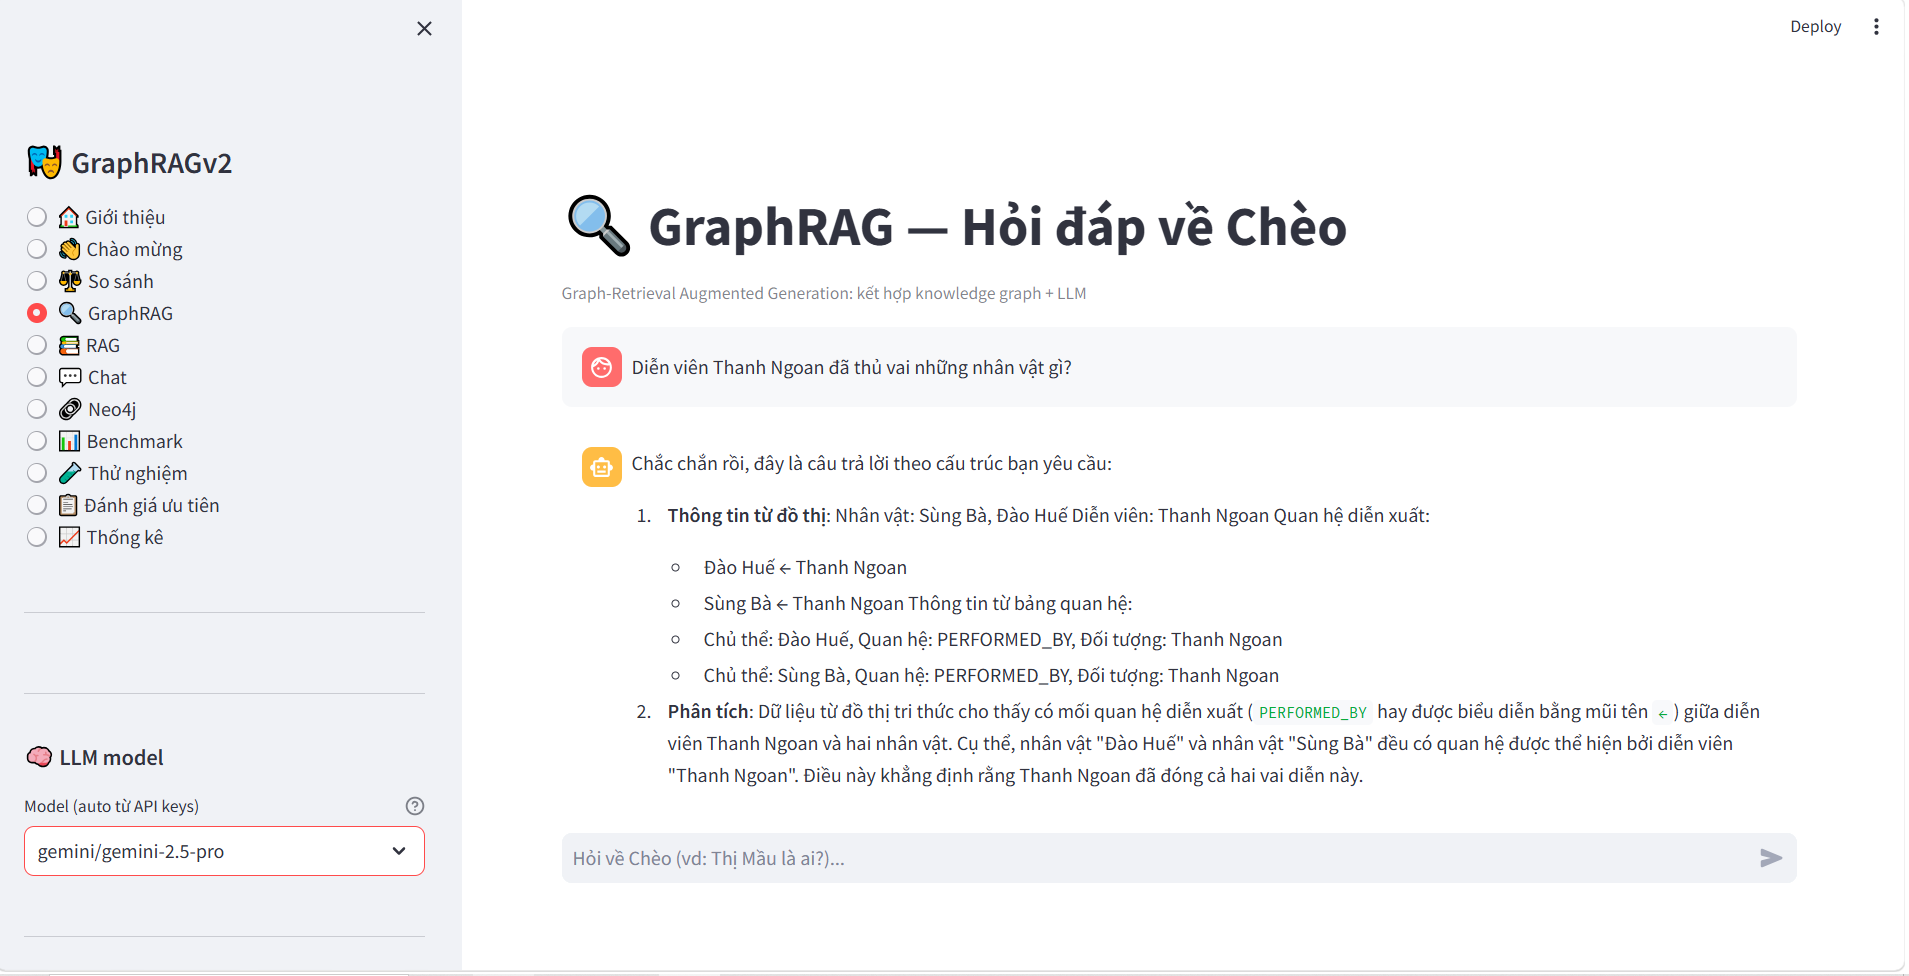
\includegraphics[width=1\linewidth]{figures//c4/UI.png}
    \caption{Giao diện thử nghiệm của hệ thống.}
    \label{fig:UI}
\end{figure}

Ở cả hai hình thức, câu trả lời của ba hệ thống được hiển thị dưới tên ẩn danh ``Hệ thống AI'', ``Hệ thống AI Plus'' và ``Hệ thống AI Pro'' thay vì tên thực (LLM-only, RAG truyền thống, GraphRAG) nhằm loại bỏ định kiến từ nhãn hiệu. Ánh xạ giữa tên hiển thị và hệ thống thật chỉ công khai cho nghiên cứu viên.

\subsection{Thiết kế kiểm nghiệm với người dùng}
\label{sec:user_study}

\subsubsection{Chấm điểm đa tiêu chí}
\label{sec:experiment_study}

Hình thức thực nghiệm đầu tiên sử dụng trang Experiment, cho phép người tham gia tự đặt câu hỏi và chấm điểm câu trả lời của ba hệ thống trong thời gian thực. Thử nghiệm tổ chức theo bốn bước: ba bước đầu yêu cầu chọn một câu hỏi trong số bảy câu chuẩn bị sẵn tại mỗi mức độ Dễ, Trung bình và Khó; bước cuối cho phép đặt một câu hỏi tự do. Thiết kế này vừa đảm bảo có câu hỏi có ground truth để so sánh giữa các người tham gia, vừa khảo sát được các câu hỏi tự phát phản ánh nhu cầu thực.

Với mỗi câu, hệ thống chạy đồng thời ba pipeline và hiển thị câu trả lời song song trong ba cột ẩn danh. Người tham gia chấm điểm từng hệ thống theo ba tiêu chí trên thang 1--5: \textit{Chính xác} (thông tin có đúng không), \textit{Đầy đủ} (bao quát nội dung câu hỏi) và \textit{Tự nhiên} (dễ đọc, mạch lạc); đồng thời chọn hệ thống tổng thể tốt nhất. Sau bốn bước, người tham gia trả lời khảo sát hậu nghiệm về mức độ hiểu biết Chèo, tần suất sử dụng công cụ AI, tiêu chí đặt nặng nhất khi lựa chọn và các loại lỗi thường gặp.

Đối tượng tham gia hình thức này là sinh viên, đại diện cho người dùng phổ thông không có kiến thức chuyên sâu về Chèo. Cách chọn đối tượng này nhằm phản ánh trải nghiệm cảm nhận của đông đảo người dùng cuối trong bối cảnh không có điều kiện thẩm định từng chi tiết tri thức. Thông tin hậu nghiệm cho phép phân tích kết quả theo các phân nhóm --- chẳng hạn nhóm có hiểu biết Chèo so với nhóm không có, hoặc nhóm sử dụng AI thường xuyên so với nhóm ít sử dụng.

\subsubsection{Đánh giá so sánh}
\label{sec:preference_study}

Hình thức thực nghiệm thứ hai sử dụng trang Preference. Hai mươi mốt câu hỏi tiêu biểu được chọn từ CheoBench v2, bao phủ cả ba nhóm độ khó và nhiều dạng truy vấn từ tra cứu trực tiếp đến phân tích liên vở. Câu trả lời của ba hệ thống đã được sinh sẵn và lưu trữ; người tham gia đọc đồng thời ba câu trả lời hiển thị ẩn danh trong ba cột, chọn câu trả lời tốt nhất và có thể ghi chú nhận xét cho từng câu.

Khác với hình thức trước, Preference không yêu cầu chấm điểm theo thang nhiều mức mà chỉ yêu cầu phán xét tổng thể ``câu trả lời nào là hay nhất''. Định dạng so sánh ba cột trực tiếp giúp người tham gia dễ phát hiện các lỗi tinh tế như chi tiết sai lệch, thiếu sót về nhân vật hoặc mâu thuẫn nội dung --- những lỗi mà các độ đo tự động thường bỏ qua. Việc sử dụng câu trả lời sinh sẵn đảm bảo công bằng: mọi người tham gia đánh giá trên cùng một tập câu trả lời, loại trừ biến động giữa các lần gọi mô hình.

Đối tượng tham gia hình thức này là các chuyên gia có hiểu biết sâu về nghệ thuật Chèo. Kiến thức chuyên môn cho phép họ thẩm định các chi tiết đặc thù của miền --- như tính chính xác của tên nhân vật, mối quan hệ giữa vở diễn, hay sự tinh tế trong cách diễn đạt --- mà người dùng phổ thông khó nắm bắt. Đánh giá của chuyên gia do đó có độ tin cậy cao hơn khi so sánh trực tiếp chất lượng nội dung giữa các hệ thống.

\subsection{Kết quả kiểm nghiệm với người dùng}

\textit{Phần này tổng hợp kết quả của cả hai hình thức kiểm nghiệm. Do quá trình thu thập dữ liệu người dùng vẫn đang tiếp tục tại thời điểm viết báo cáo, các số liệu chi tiết sẽ được bổ sung trong phiên bản hoàn chỉnh.}

% [Placeholder — cập nhật khi có dữ liệu thu thập đầy đủ]
% - Kết quả hình thức 1 (sinh viên): phân bổ phiếu hệ thống tốt nhất, điểm trung bình ba tiêu chí theo từng hệ thống, phân tích theo phân nhóm hiểu biết Chèo.
% - Kết quả hình thức 2 (chuyên gia): phân bổ phiếu chọn, phân tích định tính từ ghi chú.
% - Đối sánh giữa đánh giá sinh viên và đánh giá chuyên gia.
% - Đối sánh giữa đánh giá chủ quan và đánh giá khách quan từ các độ đo ở Mục~\ref{sec:experiments}.

\subsection{Thảo luận trải nghiệm thực tế}

\textit{Phần thảo luận chi tiết sẽ được hoàn thiện khi có đầy đủ dữ liệu kiểm nghiệm người dùng. Dự kiến các điểm thảo luận bao gồm: sự tương đồng và khác biệt giữa đánh giá chủ quan và đánh giá khách quan bằng các độ đo tự động; khác biệt trong cách đánh giá giữa nhóm sinh viên và nhóm chuyên gia; các hạn chế còn lại của hệ thống được bộc lộ qua phản hồi thực tế; và ý nghĩa ứng dụng của hệ thống trong bảo tồn và truyền bá di sản nghệ thuật Chèo.}

\section*{Tiểu kết}
\addcontentsline{toc}{section}{Tiểu kết}

Chương này trình bày quá trình hiện thực hoá và đánh giá hệ thống GraphRAG dựa trên các thiết kế ở Chương 3. Phần cài đặt đã xây dựng môi trường thực nghiệm hoàn chỉnh với Knowledge Graph trên Neo4j, pipeline GraphRAG đầy đủ và hai hệ thống tham chiếu là RAG truyền thống và LLM-only. Ba hệ thống chia sẻ cùng mô hình ngôn ngữ và cùng tham số sinh, đảm bảo chênh lệch kết quả chỉ phản ánh khác biệt về nguồn tri thức và cơ chế truy xuất.

Thực nghiệm định lượng được triển khai theo ba câu hỏi nghiên cứu, sử dụng hệ thống độ đo đa chiều bao gồm cả chất lượng truy xuất và chất lượng tạo sinh. Trên toàn bộ 100 câu hỏi của CheoBench v2, GraphRAG đạt điểm tổng hợp $S_{\text{overall}} = 0{,}835$ so với $0{,}595$ của RAG truyền thống, với khoảng cách lớn nhất rơi vào các độ đo ngữ nghĩa --- Context Recall chênh +0,545 và Faithfulness chênh +0,252. Thí nghiệm ablation theo mức độ truy xuất trên 20 câu phân tầng cho thấy cấu hình kết hợp đa mức độ đạt $S_{\text{overall}} = 0{,}811$, vượt cấu hình đơn lẻ tốt nhất một khoảng +0,139 điểm, khẳng định thiết kế truy xuất đa mức độ là thành phần then chốt của kiến trúc.

Ở bước triển khai, hệ thống được đưa lên hạ tầng đám mây và kiểm nghiệm với người dùng qua hai hình thức thực nghiệm: chấm điểm đa tiêu chí và đánh giá so sánh. Cách thiết kế này cho phép thu thập phản hồi ở cả mức chi tiết từng tiêu chí lẫn mức phán xét tổng thể, bổ sung cho đánh giá định lượng ở khía cạnh chất lượng chủ quan. Tổng hợp các kết quả trên tạo cơ sở cho những đánh giá tổng kết và hướng phát triển được trình bày trong chương tiếp theo.
